\documentclass[doktyp=semarbeit, sprache=german]{TUBAFarbeiten}
\usepackage[utf8]{inputenc}
\usepackage[T1]{fontenc}
\usepackage{graphicx} 
\usepackage{amsmath}
\usepackage{subcaption}
\usepackage{booktabs}
\usepackage{url}
\usepackage{listings}
\usepackage{xcolor}
\usepackage[Algorithmus]{algorithm}
\usepackage{algorithmicx}
\usepackage[noend]{algpseudocode}
\usepackage{float}

\definecolor{codegreen}{rgb}{0,0.6,0}

\lstset{
  language=bash,
  basicstyle=\ttfamily
}
\lstnewenvironment{CPP}
  {\lstset{language=C++,basicstyle=\ttfamily\small,frame=none,extendedchars=false,showstringspaces=false,tabsize=4,commentstyle=\color{codegreen},
    keywordstyle=\color{blue},
    numberstyle=\tiny\color{orange},
    stringstyle=\color{gray}}}
  {}
\captionsetup{compatibility=false}
\bibliographystyle{unsrt}
\TUBAFFakultaet{Fakultät für Mathematik und Informatik}
\TUBAFInstitut{Institut für Informatik}
\TUBAFLehrstuhl{Lehrstuhl für Betriebssysteme und Kommunikationstechnologien}
\TUBAFTitel{Aufbau eines Prototyps für verteilte CUDA Programmierung}
\TUBAFUntertitel{Development of a prototype for distributed CUDA programming}
\TUBAFKorrektor{Dr. rer. nat. Martin Reinhardt}
\TUBAFBetreuer{Prof. Dr. Konrad Froitzheim}
\TUBAFAutor[S. Dressel]{Samuel Dressel}
\TUBAFStudiengang{Angewandte Informatik}
\TUBAFVertiefung{Parallelrechner}
\TUBAFMatrikel{59963}
\TUBAFDatum{\today}
\begin{document}
\maketitle
\tableofcontents
\TUBAFErklaerungsseite
\newpage
\section{Einleitung}
Egal ob in Forschung, Industrie oder Dienstleistung - alle Bereiche verwenden mehr und mehr komplexe Algorithmen, um Abläufe und Dienste zu planen, zu koordinieren oder durchzuführen. Mit der steigenden Rechenleistung in den vergangenen Jahrzehnten können diese auch auf schon einfachen Geräten ausgeführt werden. Jedoch gibt es nach wie vor eine Vielzahl von Algorithmen, die bei steigender Größe des behandelten Problems viel Rechenzeit bzw. -leistung benötigen. Um diese Algorithmen effizienter zu gestalten, werden diese meist auf einem Rechnerverbund bzw. Cluster ausgeführt. Klassisch bestehen diese sogenannten \textit{High Performance Computing Cluster} aus mehreren Knoten mit jeweils eigenen Prozessoren. Dabei wird die zu bearbeitende Aufgabe (Job) letztendlich auf die Knoten aufgeteilt; die Berechnung erfolgt auf den dazugehörigen CPUs. Sind die zu erledigenden Aufgaben ziemlich groß bei verhältnismäßig einfachen Recheninstruktionen, so kann die Compute-Zeit je nach Setup trotzdem relativ hoch sein. Dies hängt damit zusammen, dass eine moderne CPU zwar auch komplexere Instruktionen schnell bearbeiten kann, jedoch nach wie vor unter 100 Kerne besitzt.
\\\\Im Gegensatz zu herkömmlichen Prozessoren stehen hier Grafikprozessoren, die im Hinblick auf ihre Architektur wesentlich anders aufgebaut sind. Moderne GPUs besitzen oft mehrere tausend Kerne, wenn auch nur mit einem jeweils einfachen Set an möglichen Instruktionen. Diese Eigenschaft lässt sich ausnutzen, um bestimmte Probleme in einem Bruchteil der auf einer CPU benötigten Rechenzeit zu bewältigen. Wie CPUs lassen sich auch mehrere GPUs miteinander verbinden, um eine weitere Beschleunigung zu erzielen. Dabei sind jedoch sowohl beim technischen Setup als auch bei der Implementierung eines Algorithmus zur Ausführung auf mehreren Grafikchips gewisse Dinge zu beachten.
\\\\In dieser Arbeit soll auf die Grundlagen des verteilten Computings mit mehreren GPUs eingegangen und eine Art Handbuch für den Aufbau eines Prototyps mit mehreren NVIDIA-Grafikchips gegeben werden. Dabei werden zunächst in Kapitel 2 die benötigten Schnittstellen MPI und CUDA erläutert. In Kapitel 3 findet sich dann eine schrittweise Anleitung für den technischen Aufbau und die Konfiguration des Prototyps. Anschließend wird in Kapitel 4 auf das Benchmarking des Prototyps eingegangen und in Kapitel 5 ein Fazit gegeben.
\newpage
\section{Grundlagen}
\subsection{Message-Passing-Interface (MPI)}
Das Message-Passing-Interface, kurz MPI, ist eine standartisierte Schnittstelle für die Kommunikation auf verteilten Systemen. Es wird häufig in wissenschaftlichen und ingenieurstechnischen Domänen verwendet, um größere Problemstellungen effizienter zu bearbeiten und zu lösen \cite{MPIBook}. MPI ist speziell für die Verwendung auf verteilten Systemen mit ebenso verteiltem Speicher konstruiert. Dabei kann jeder Prozessor, der Teil der Bearbeitung eines Workloads ist, nur auf seinen lokalen Speicher zugreifen. Es können jedoch durch Messages Daten von einem lokalen Speicher in den anderen übertragen werden.
\\MPI ist als Bibliothek implementiert, nicht als Programmiersprache. Dabei existieren Implementierungen für zahlreiche Programmiersprachen wie C, C++, Python oder Fortran \cite{ScriptPC}.
\\Die grundlegendste Art der Kommunikation findet zwischen zwei Prozessen statt. Dabei übermittelt ein Sendeprozess Informationen an einen Empfangsprozess.
\begin{figure}
	\centering
	\captionsetup{justification=centering} 
	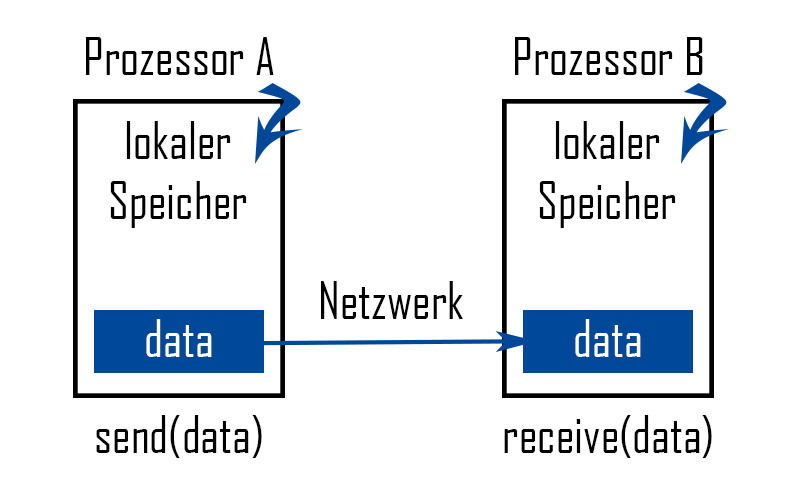
\includegraphics[width=1.0\textwidth]{images/MPIModell.jpg}
	\caption{Grundlegendes Konzept von MPI: Ein Sendeprozess sendet Daten an einen Empfangsprozess über ein Netzwerk. Jeder Prozess kann nur unmittelbar auf seinen zugehörigen lokalen Speicher zugreifen.}
	\label{img:mpimodell}
\end{figure}
Prozesse lassen sich außerdem in Gruppen zusammenfassen, wobei jeder Prozess eine eindeutige Nummer (Rang bzw. Rank) zugeordnet wird. Der Zugriff auf diese Gruppe wird über einen Kommunikator gesteuert. Innerhalb dieser Gruppe können mithilfe einer Broadcast-Operation von einem Masterprozess allen anderen Prozessen Nachrichten gesendet werden. Die zurückgegebenen Daten werden mithilfe einer Gather-Funktion wieder eingesammelt.
\\Dieses Konzept wird auch für den im Rahmen dieser Arbeit erstellten Minicluster genutzt: Der Workload wird von dem Masterknoten definiert und dann über das Message-Passing-Interface an die Work-Nodes (Arbeitsknoten) gesendet. Dies erlaubt dann letztendlich die Verteilung der Workload innerhalb des Clusters.
\subsection{CUDA}
Im Vergleich zu einer CPU besteht eine Grafikkarte aus einer großen Anzahl parallel nutzbarer Kerne, die eine Vielzahl von Berechnungen parallel ausführen können. Beispielsweise besitzt eine \textit{NVIDIA RTX 2080} 2944 CUDA-Kerne, während die meisten CPUs 8 bis 16 Kerne besitzen \cite{RTXCores}. 
Natürlich sind die Kerne einer GPU in ihrer Struktur und Instruktionskomplexität wesentlich einfacher, da sie dafür ausgelegt sind, Aufgaben als Gruppe zu bearbeiten.
Eine CPU ist auf generelle Programmanforderungen ausgelegt und muss eine Vielzahl von Befehlen und Datentypen unterstützen. Eine GPU ist hingegen auf Grafikberechnungen spezialisiert und in ihrer grundlegenden Funktion für Pixelberechnungen konzipiert worden.
\\Aufgrund dieser Struktur lassen sich GPUs aber nicht nur für Grafikberechnungen nutzen, sondern auch bei der Berechnung von wissenschaftlichen Problemen.
Um diese Architektur nutzen und steuern zu können, wurde die Programmierschnittstelle CUDA (\textit{Compute Unified Device Architecture}) entwickelt. CUDA wurde dabei von NVIDIA entwickelt und erlaubt die Beschleunigung von Programmen, indem neben der CPU bestimmte Programmteile von einer oder mehreren GPUs parallelisiert bearbeitet werden.
\\CUDA besitzt Bindings für viele wissenschaftlich genutzte Programmiersprachen wie C/C++, Fortran oder Python und ist mit allen herkömmlichen Betriebssystemen kompatibel \cite{CUDADefinition}.
\subsection{CUDA und MPI}
Sowohl CUDA als auch MPI dienen in ihrer grundlegenden Funktion zur Bereitstellung einer Schnittstelle von parallelen bzw. verteilten Berechnungen. MPI erlaubt es wie schon oben erwähnt, bestimmte Aufgaben innerhalb eines verteilten Systems zu koordinieren und aufzuteilen. Grundsätzlich wird dabei nur die Rechenleistung der einzelnen CPUs genutzt \cite{CUDAAwareMPI}.
Für eine weitere Optimierung durch die Verwendung von verschiedenen GPUs in einem verteilten System ist zusätzlich CUDA als GPU-Schnittstelle notwendig.
Dabei ergibt sich jedoch folgendes Problem: Standartmäßig werden bei der Verwendung von MPI nur Zeiger auf den Hauptspeicher des Hosts weitergeleitet. Jedoch müssen bei der Kombination von MPI und CUDA meist GPU-Buffer gesendet werden. Hierzu müssen diese Buffer zunächst in den Hauptspeicher kopiert werden, um dann gesendet werden zu können:
\begin{CPP}
//MPI rank 0
cudaMemcpy(s_buf_h,s_buf_d,size,cudaMemcpyDeviceToHost);
MPI_Send(s_buf_h,size,MPI_CHAR,1,100,MPI_COMM_WORLD);

//MPI rank 1
MPI_Recv(r_buf_h,size,MPI_CHAR,0,100,MPI_COMM_WORLD, &status);
cudaMemcpy(r_buf_d,r_buf_h,size,cudaMemcpyHostToDevice);
\end{CPP}
Diese Tatsache führt zu erheblichen Zeitverlusten und kann eine Optimierung von Berechnung mit CUDA und MPI einschränken. Daher wurde eine Vielzahl von MPI-Implementation wie \textit{MVAPICH2} oder \textit{OpenMPI} um eine spezielle CUDA-Unterstützung erweitert. Diese Unterstützung trägt den Namen \textit{CUDA-aware MPI}. Mit CUDA-aware MPI können GPU-Buffer direkt an MPI weitergegeben werden:
\begin{CPP}
//MPI rank 0
MPI_Send(s_buf_d,size,MPI_CHAR,1,100,MPI_COMM_WORLD);

//MPI rank n-1
MPI_Recv(r_buf_d,size,MPI_CHAR,0,100,MPI_COMM_WORLD, &status);
\end{CPP}
Dabei muss eine CUDA-aware MPI-Implementation unterscheiden, ob der jeweilige Buffer auf dem Hostspeicher oder dem Speicher der GPU liegt. Seit der CUDA-Version 4.0 wurde das CUDA-Feature UVA (\textit{Unified Virtual Addressing}) eingeführt, welches den Hauptspeicher und den Gerätespeicher kombiniert und in einem virtuellen Adressraum zusammenfasst.
\begin{figure}
	\centering
	\captionsetup{justification=centering} 
	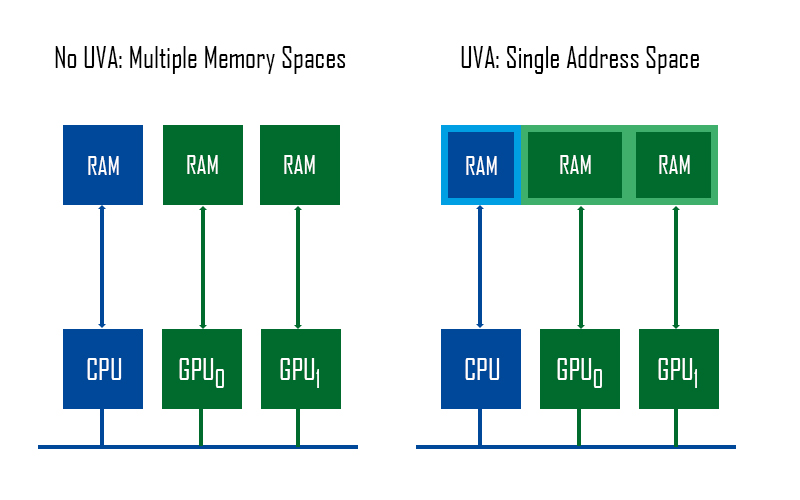
\includegraphics[width=1.0\textwidth]{images/CUDAUVA.jpg}
	\caption{Links ist das Speicherhandling ohne UVA abgebildet, rechts das Speicherhandling mit UVA. Bei der Nutzung von Unified Virtual Addressing werden die Speicherräume aller System- und Gerätespeicher in einem virtuellen Adressraum zusammengefasst.}
	\label{img:cudauval}
\end{figure}
Ein weiteres Feature von CUDA, eingeführt mit der Version 5.0, ist die \textit{GPUDirect}-Funktionalität. Dies erlaubt mithilfe des \textit{Remote Direct Memory Access} (RDMA) das direkte Senden von Grafikspeicher an den Netzwerkadapter ohne Routing über den jeweiligen Hauptspeicher. 
Diese Funktionen bilden die Grundlage für eine gelungene Optimierung von verteilten Berechnungen auf verteilten Systemen durch Nutzung von CUDA-aware MPI.
\section{Technischer Aufbau und Konfiguration}
Für den Aufbau des Mini-Clusters werden zunächst folgende Dinge benötigt \cite{ClusterSetup}:
\begin{itemize}
	\item Nvidia Jetson Nano (3x)
	\item SD-Karte (3x)
	\item Ethernet-Kabel (4x)
	\item 4-Port Ethernet Switch
	\item Optional: 40mm Lüfter (3x, in diesem Fall wurde der Noctua NF-A4x20 verwendet)
\end{itemize}
Der technische Aufbau beginnt mit der physischen Verbindung der Nvidia Jetson Nanos. Dazu werden diese alle via Ethernet-Kabel mit einem Ethernet-Switch verbunden, welcher wiederum durch Ethernet mit einem Router und dadurch mit dem Internet verbunden ist. An sich benötigt der Cluster keinen Internetzugang, für die Einrichtung ist dieser jedoch unersetzlich. Einer der Jetson Nanos dient dabei als Head-Node (Masterknoten), die anderen zwei als Worker-Nodes.
\\Ist das physische Setup abgeschlossen, wird als nächstes auf jedem der Jetson Nanos das \textit{Jetson Nano Developer Kit SD Card Image} installiert. Dies geschieht durch das Schreiben des Images auf die jeweilige SD-Karte und einem anschließenden Setup auf den Jetson Nanos \cite{SDImage}. Danach wird das System durch Aktualisierung der Pakete auf den neuesten Stand gebracht:
\begin{lstlisting}
sudo apt-get update
sudo apt-get upgrade
\end{lstlisting}
Es folgt die Installation des \texttt{nano}-Texteditors und des SSH-Paketes. Dabei ist SSH für den Remotezugriff auf die einzelnen Knoten notwendig; an Stelle des \texttt{nano}-Texteditors kann alternativ jeder andere Editor benutzt werden.
\begin{lstlisting}
sudo apt-get install nano
sudo apt-get install openssh-server
\end{lstlisting}
Zusätzlich ist auf dem Masterknoten der NFS-Kernel-Server zu installieren:
\begin{lstlisting}
sudo apt-get install nfs-kernel-server
\end{lstlisting}
Auf den Worker-Nodes wird dagegen das \texttt{nfs-common}-Paket installiert:
\begin{lstlisting}
sudo apt-get install nfs-common
\end{lstlisting}
NFS und die damit verbundenen Pakete sind notwendig, um später Dateien innerhalb des Clusters auszutauschen.
\\Um den Cluster nun einzurichten, muss zunächst jedem der drei Knoten eine statische IP zugewiesen werden. Dies erfolgt entweder über die Netzwerkeinstellungen oder über das Bearbeiten der Interface-Datei:
\begin{lstlisting}
cd /etc/network
sudo nano interfaces
\end{lstlisting}
Dafür werden der Datei folgende Zeilen hinzugefügt:
\begin{lstlisting}
auto eth0
iface eth0 inet static
address 192.168.178.10
gateway 192.168.178.1
netmask 255.255.255.0
\end{lstlisting}
Dabei ist die Adresse \texttt{192.168.178.10} die Adresse des Masterknotens, die Worker-Nodes erhalten dann dementsprechend die IP-Adressen \texttt{192.168.178.11} und \texttt{192.168.178.12}. Damit die Änderungen wirksam werden, müssen entweder die Jetson Nanos oder der Network-Service neugestartet werden.
\\Als nächstes erfolgt die Einrichtung von SSH innerhalb des Clusters. Dazu wird zuerst jedem Knoten ein Name zur besseren Identifikation zugewiesen. Hierfür wird die \texttt{hostname}-Datei bearbeitet:
\begin{lstlisting}
sudo nano /etc/hostname
\end{lstlisting}
Der Masterknoten erhält in diesem Fall den Namen \texttt{master}, die Worker-Nodes die Namen \texttt{slave1} und \texttt{slave2}. Als nächstes werden in der \texttt{hosts}-Datei die statischen IP-Adressen aller Knoten hinzugefügt. Dies geschieht wie der vorige Schritt auf allen Knoten:
\begin{lstlisting}
sudo nano /etc/hosts
\end{lstlisting}
Die \texttt{hosts}-Datei sollte dann so aussehen:
\begin{lstlisting}
192.168.178.10 master
192.168.178.11 slave1
192.168.178.12 slave2
\end{lstlisting}
Nach dem Einrichten der statischen IP-Adressen folgt nun das Setup von SSH. Dazu wird zunächst ein 2048-bit RSA Schlüsselpaar auf dem Masterknoten erstellt:
\begin{lstlisting}
ssh-keygen -t rsa -b 2048
\end{lstlisting}
Danach wird die SSH ID an alle Knoten inklusive des Masterknotens weitergeben:
\begin{lstlisting}
ssh-copy-id master
ssh-copy-id slave1
ssh-copy-id slave2
\end{lstlisting}
Eine Kommunikation zwischen den Knoten ohne ständige Passwort- bzw. Berechtigungsabfrage ist für die Funktionalität des Cluster von großer Bedeutung. Dies geschieht durch das Generieren der \texttt{known\_hosts}-Datei im \texttt{.ssh}-Ordner.  Dazu wird zunächst eine Datei mit den Namen aller Knoten im \texttt{.ssh}-Ordner angelegt:
\begin{lstlisting}
cd .ssh
sudo nano name_of_hosts
\end{lstlisting}
Die Datei enthält dann folgende Einträge:
\begin{lstlisting}
master
slave1
slave2
\end{lstlisting}
Damit der \texttt{ssh-keyscan} die Datei lesen kann, müssen anschließend die Zugriffsberechtigungen geändert werden:
\begin{lstlisting}
sudo chmod 666 ~/.ssh/name_of_hosts
\end{lstlisting}
Mit folgendem Befehl wird letztendlich die \texttt{known\_hosts}-Datei erzeugt:
\begin{lstlisting}
ssh-keyscan -t rsa -f ~/.ssh/name_of_hosts >~/.ssh/known_hosts
\end{lstlisting}
Als letztes muss diese Datei und die notwendigen Schlüssel noch an die anderen Knoten kopiert werden:
\begin{lstlisting}
cd .ssh
scp known_hosts id_rsa id_rsa.pub nvidia@master:.ssh
scp known_hosts id_rsa id_rsa.pub nvidia@slave1:.ssh
scp known_hosts id_rsa id_rsa.pub nvidia@slave2:.ssh
\end{lstlisting}
Der letzte Schritt der Konfiguration ist das Erstellen und Mounten eines gemeinsamen Arbeitsordners für alle Knoten. Hierfür das Network File System benutzt, dessen Pakete anfangs installiert wurden. Auf dem Masterknoten wird dabei als erstes dieser Arbeitsordner erstellt:
\begin{lstlisting}
sudo mkdir /cloud
\end{lstlisting}
Danach muss die \texttt{exports}-Datei auf dem Masterknoten editiert werden:
\begin{lstlisting}
sudo nano /etc/exports
\end{lstlisting}
Diese Datei enthält alle Informationen über das Exportieren des Arbeitsordners auf die einzelnen Knoten:
\begin{lstlisting}
/cloud slave1(rw,sync,no_root_squash,no_subtree_check)
/cloud slave2(rw,sync,no_root_squash,no_subtree_check)
\end{lstlisting}
Die zwei Worker-Nodes müssen nun diesen gemeinsamen Arbeitsordner mounten. Dazu wird auf jedem Worker-Node der \texttt{cloud}-Ordner erstellt und mithilfe des Editierens der \texttt{fstab}-Datei gemountet:
\begin{lstlisting}
sudo mkdir /cloud
sudo nano /etc/fstab

master:/cloud /cloud nfs rsize=8192,wsize=8192,timeo=14,intr
\end{lstlisting}
Alternativ lässt sich ein gemeinsamer Arbeitsordner auch manuell mounten:
\begin{lstlisting}
sudo mount master:/cloud /cloud
\end{lstlisting}
Je nach verwendetem Linuxbetriebssystem muss nun noch sichergestellt werden, dass das CUDA-Toolkit sowie MPI mit Cuda-Unterstützung installiert ist. Das Cuda-Toolkit kann über die offizielle Website heruntergeladen werden (\cite{CudaToolkit}); bei der Konfiguration und Installation von MPI muss je nach Implementierung die Cuda-Unterstützung manuell eingestellt werden.
\\\\Der technische Aufbau und die Konfiguration des Clusters ist an dieser Stelle abgeschlossen. Wird wie in dieser Arbeit ebenfalls betrachtet ein weiteres cudafähiges Gerät in den Minicluster eingebunden, so geschieht die Konfiguration analog dieser Schrittfolge.
\section{Benchmarking und Test ausgewählter Algorithmen}
In diesem Kapitel soll die Implementierung ausgewählter Algorithmen vorgestellt und mit verschiedenen Setups getestet und ausgewertet werden.
\subsection{Einfache Vektoraddition}
Um das Zusammenspiel von Cuda und MPI besser zu verstehen, wird zunächst ein einfacher Algorithmus zur Vektoraddition betrachtet. Der Quellcode findet sich dabei in Anhang B. Im wesentlichen geschieht bei der implementierten Vektoraddition mithilfe von Cuda und MPI folgendes: Zunächst wird MPI standartmäßig initialisiert. Dann wird überprüft, ob die angegeben MPI-Hosts cudafähige Geräte besitzen und wenn ja, wie viele. Nach der Allokieren des Speichers auf dem Host und dem Initalisieren der beiden Vektoren wird der Speicher für die verteilte Berechnung allokiert. Dies geschieht in diesem Fall nicht durch eine einfache Allokierung mit \texttt{cudaMalloc}, sondern durch \texttt{cudaMallocManaged}. Dies bewirkt die Verwendung von dem sogenannten \textit{Unified Memory} \cite{UnifiedMemory}. Unified Memory stellt einen einzelnen Speicheradressraum für alle Prozessoren in einem System bereit. Der Zugriff der einzelnen Prozessoren (in diesem Fall die einzelnen Grafikprozessoren) auf den Speicher wird durch Cuda selbst gehandhabt.
\\Nach der Allokierung des Speichers erfolgt die Aufteilung der Vektoraddition auf die einzelnen Grafikprozessoren durch die Scatterfunktionalität von MPI. Anschließend folgt der Aufruf des Kernels. Die Aufteilung auf den einzelnen Prozessoren an sich erfolgt in diesem Fall durch eine sogenannte Grid-Stride-Loop (siehe \cite{GridStride}).
\\\\Für das Benchmarking dieses Algorithmus ist nun die Zeit interessant, welche der Kernel benötigt und welche das Programm an sich insgesamt benötigt. Eine Zusammenfassung von generierten Ergebnissen ist in der nachfolgenden Tabelle \ref{tab:addition} ersichtlich.
\begin{table}[]
\centering
\resizebox{\textwidth}{!}{%
\begin{tabular}{@{}ccccccccc@{}}
\multicolumn{1}{c|}{}            & \multicolumn{2}{c|}{1 GPU - 1 Rank}         & \multicolumn{2}{c|}{1 GPU - 4 Ranks}         & \multicolumn{2}{c|}{3 GPUs - 3 Ranks}        & \multicolumn{2}{c|}{4 GPUs - 4 Ranks} \\
\multicolumn{1}{c|}{Vektorgröße} & Zeit Kernel & \multicolumn{1}{c|}{Zeit MPI} & Zeit Kernel & \multicolumn{1}{c|}{Zeit MPI}  & Zeit Kernel & \multicolumn{1}{c|}{Zeit MPI}  & Zeit Kernel        & Zeit MPI         \\ \midrule
\multicolumn{1}{c|}{5 000 000}   & 26.3 ms     & \multicolumn{1}{c|}{288 ms}   & 7.9 ms      & \multicolumn{1}{c|}{1158.2 ms} & 24.8 ms     & \multicolumn{1}{c|}{7405.1 ms} & 27.1 ms            & 10935.5 ms       \\
\multicolumn{1}{c|}{10 000 000}  & 44.1 ms     & \multicolumn{1}{c|}{516 ms}   & 22.5 ms     & \multicolumn{1}{c|}{1850.6 ms} & 34.3 ms     & \multicolumn{1}{c|}{14691 ms}  & 32.4 ms            & 21829.1 ms       \\
\multicolumn{1}{c|}{15 000 000}  & 51.3 ms     & \multicolumn{1}{c|}{743 ms}   & 48.7 ms     & \multicolumn{1}{c|}{2746.2 ms} & 67.6 ms     & \multicolumn{1}{c|}{22092 ms}  & 45.2 ms            & 32592.9 ms       \\
\multicolumn{1}{c|}{20 000 000}  & 74.5 ms     & \multicolumn{1}{c|}{977.4 ms} & 52.5 ms     & \multicolumn{1}{c|}{4670.4 ms} & 70.2 ms     & \multicolumn{1}{c|}{29351 ms}  & 62.7 ms            & 43554.5 ms       \\ \midrule
\multicolumn{9}{l}{}                                                                                                                                                                                                
\end{tabular}%
}
\caption{Übersicht der Ergebnisse des Benchmarkings des Vektoradditionsalgorithmus. Verglichen wurden hier vier verschiedene Setups: Zuerst wurde der Algorithmus mit einem Rank auf einem Jetson Nano getestet, dann mit vier Ranks auf einem Jetson Nano. Bei dem Test mit 3 GPUs handelt es um drei Nvidia Jetson Nanos; bei dem Test mit 4 GPUs um drei Nvidia Jetson Nanos und einen Nvidia Jetson TX2.}
\label{tab:addition}
\end{table}
\\Betrachet man die Kernel Zeiten, so lässt sich feststellen, dass die insgesamte Laufzeit bei der Verwendung eines Grafikprozessors mit einem Rank am Besten ist und die benötigte Kernel-Zeit bei der Verwendung eines Grafikprozessors mit vier Ranks am Besten ist. Die Zeit, welche die Zuhilfenahme von anderen Grafikprozessoren zur Lösung des Problems benötigt, ist wesentlich höher.
Dennoch lassen sich in diesem Fall die Vorteile und die Nachteile der gewählten Implementierung erkennen. Das Problem der Vektoraddition ist von seiner Komplexität sehr gering. Somit kann insgesamt weniger Zeit durch die Verwendung von mehreren Grafikprozessoren eingespart werden als durch die Datenübertragungszeit von MPI und durch das automatisierte Speichermanagement von Cuda durch die Verwendung von Unified Memory erzeugt wird. Man sieht das beispielsweise bei Vergleich der Benchmarking-Zeiten von einem Grafikprozessor mit einem MPI-Rank und der von einem Grafikprozessor mit vier MPI-Ranks. Bei der Verwendung von vier Ranks benötigt der Kernel teilweise nur ein Viertel der Zeit (statt $26.3\,ms$ nur $7.9\,ms$ bei einer Vektorgröße von $5 000 000$). Gleichzeitig ist die gesamte Laufzeit viermal so hoch.
\subsection{Floyd-Warshall-Algorithmus}
Um den Mini-Cluster ausführlicher zu testen und die Prinzipien der verteilten Berechnung mit MPI und Cuda zu veranschaulichen, wurde der Floyd-Warshall Algorithmus implementiert. Dieser Algorithmus ist Bestandteil der Graphentheorie und wurde nach Robert Floyd und Stephen Warshall benannt. Dabei löst dieser Algorithmus das Problem, in einem Knotennetz mit gegebenen Gewichtungen der Kanten die minimalen Distanzen zwischen den Städten zu finden. Das Prinzip des Floyd-Warshall-Algorithmus ist die dynamische Programmierung. Das heißt, dass alle möglichen Pfade zwischen allen Paaren von Knoten schrittweise verglichen werden und letztendlich nur die besten Werte gespeichert werden \cite{Floyd}.
\\Mathematisch lässt sich der Algorithmus folgendermaßen ausdrücken \cite{WikiFloyd}: Es sei ein Graph $G$ mit einer Gewichtsmatrix $w$. Dabei ist $w[i,j]$ das Gewicht der Kante von $i$ nach $j$, falls eine solche Kante existiert. Falls es keine Kante von $i$ nach $j$ gibt, so ist $w[i,j]$ unendlich. Mit diesen Angaben lässt sich nun eine Matrix $d$ mit den kürzesten Distanzen bestimmten:
\newpage
\begin{algorithm}
\caption{Floyd-Warshall-Algorithmus}
\label{alg:floyd}
\begin{algorithmic}[1]
\State \textbf{Gegeben}: Graph $G$ mit Gewichtungsmatrix $w$;
\State $n = |V(G)|$
\State Für alle $i,j: d[i,j] = w[i,j]$
\For{$k = 1$ bis $n$}
\For{jedes Paar $i,j$}
\State $d[i,j] = min(d[i,j], d[i,k] + d[k,j])$
\EndFor
\EndFor
\end{algorithmic}
\end{algorithm}
Der Floyd-Warshall Algorithmus hat eine Komplexität von $O(n^3)$, da die Zahl der Paare $(i,j$ quadratisch beschränkt ist.
Zunächst wurde eine serielle nicht parallele Version des Algorithmus implementiert und auf einem der Jetson Nanos getestet. Die benötigten Rechenzeiten finden sich in Tabelle \ref{tab:seriell}.
\begin{table}[]
\centering
\begin{tabular}{@{}ccccc@{}}
\multicolumn{1}{c|}{Anzahl Knoten} & 7     & 8      & 9       & 10       \\ \midrule
\multicolumn{1}{c|}{Zeit}          & 48 ms & 389 ms & 3252 ms & 24592 ms \\
\multicolumn{5}{c}{}                                                    
\end{tabular}
\caption{Rechenzeit der seriellen Implementierung des Floyd-Warshall-Algorithmus}
\label{tab:seriell}
\end{table}
\\Es wird hier sehr deutlich, dass die Rechenzeit bei einem Graphen mit 7 Knoten noch akzeptabel ist, aber mit jedem weiteren Knoten um ein Vielfaches ansteigt. Mit diesen Zeiten als Vergleich wurde nun eine parallele Version des Floyd-Warshall-Algorithmus implementiert. Der Quellcode dazu befindet sich in dem für diesen Projekt erstelltem Git-Repository \cite{Git}. Die benötigten Zeiten und eine grafische Veranschaulichung finden sich in der untenstehenden Tabelle \ref{tab:parallelfloyd} und den nachfolgenden Diagrammen \ref{img:dia1} und \ref{img:dia2}. 
\\Es wurde im Rahmen des Benchmarks jeweils mit einer Knotenanzahl von 7 bis 12 Knoten getestet; dabei wurden jeweils drei Versuche durchgeführt und für die ermittelten Zeiten der Mittelwert gebildet. Desweiteren wurde der Algorithmus in vier verschiedenen Szenarien getestet. Zunächst wurde selbiger auf einem Nvidia Jetson Nano mit einem MPI-Rank und mit 4 MPI-Ranks ausgeführt. Danach wurde der Algorithmus im Cluster mit drei Jetson Nanos und letztendlich mit einem zusätzlichen Nvidia Jetson TX2 getestet. Die gesamte Prozedur wurde insgesamt einmal mit einer Blockgröße von 16x16 und einmal mit einer Blockgröße von 256x256 durchgeführt. 
\\Bei der Betrachtung der Ergebnisse fällt als erstes auf, dass die benötigte Rechenzeit sich bei den zwei gewählten Blockgrößen gegensätzlich verhält. Bei einer Blockgröße von 16x16 erzielt das Setup mit vier Geräten und einer Knotenzahl von 12 die besten Zeiten, bei einer Blockgröße von 256x256 das Setup mit einem Gerät und einem Rank. Insgesamt lässt sich durch die Erhöhung der Blockgröße ein wesentlich besseres Ergebnis erzielen. Es fällt außerdem auf, dass bei einer kleinen Problemgröße die Verwendung eines Gerätes und eines Ranks wesentlich bessere Ergebnisse aufzeigt als bei der Nutzung von mehreren Geräten bzw. Ranks. Dies lässt sich auf die durch Verwendung von MPI entstehenden Kommunikationszeiten zurückführen. Desweiteren kommt hier auch die zusätzliche Zeit durch das erweiterte Speichermanagement hinzu. Steigt die Problemgröße dagegen, so benötigt die Ausführung im Mini-Cluster mit vier Geräten, einer Knotenanzahl von 12 und einer Blockgröße von 16x16 nur ein Viertel der Zeit, die bei einer Ausführung auf einem Gerät mit einem Rank benötigt wird.
\\Zusammenfassend lässt sich feststellen, dass die Verwendung von mehreren Geräten bei steigender Problemgröße auszahlt. Bei einer kleinen Problemgröße werden die durch MPI entstehenden Latenzzeiten zum Nachteil. Es gilt deshalb hier jeweils die Anzahl der Geräte und Ranks je nach Problem und des Größen abzuwägen.
\newpage
\begin{table}[]
\centering
\resizebox{\textwidth}{!}{%
\begin{tabular}{@{}ccccc@{}}
\toprule
\multicolumn{5}{c}{Blockgröße 16x16}                                                                             \\ \midrule
\multicolumn{1}{c|}{}                   & 1 GPU - 1 Rank & 1 GPU - 4 Ranks & 3 GPUs - 3 Ranks & 4 GPUs - 4 Ranks \\ \midrule
\multicolumn{1}{c|}{Zeit für 7 Knoten}  & 54 ms          & 125 ms          & 80 ms            & 114 ms           \\
\multicolumn{1}{c|}{Zeit für 8 Knoten}  & 93 ms          & 135 ms          & 183 ms           & 241 ms           \\
\multicolumn{1}{c|}{Zeit für 9 Knoten}  & 448 ms         & 1139 ms         & 436 ms           & 535 ms           \\
\multicolumn{1}{c|}{Zeit für 10 Knoten} & 2002 ms        & 1362 ms         & 1539 ms          & 1488 ms          \\
\multicolumn{1}{c|}{Zeit für 11 Knoten} & 11494 ms       & 7988 ms         & 4106 ms          & 4712 ms          \\
\multicolumn{1}{c|}{Zeit für 12 Knoten} & 89402 ms       & 61916 ms        & 22491 ms         & 17067 ms         \\ \midrule
\multicolumn{5}{l}{}                                                                                             \\ \midrule
\multicolumn{5}{c}{Blockgröße 256x256}                                                                           \\ \midrule
\multicolumn{1}{c|}{}                   & 1 GPU - 1 Rank & 1 GPU - 4 Ranks & 3 GPUs - 3 Ranks & 4 GPUs - 4 Ranks \\ \midrule
\multicolumn{1}{c|}{Zeit für 7 Knoten}  & 10 ms          & 91 ms           & 73 ms            & 105 ms           \\
\multicolumn{1}{c|}{Zeit für 8 Knoten}  & 14 ms          & 135 ms          & 150 ms           & 218 ms           \\
\multicolumn{1}{c|}{Zeit für 9 Knoten}  & 53 ms          & 215 ms          & 464 ms           & 523 ms           \\
\multicolumn{1}{c|}{Zeit für 10 Knoten} & 113 ms         & 388 ms          & 1201 ms          & 1343 ms          \\
\multicolumn{1}{c|}{Zeit für 11 Knoten} & 280 ms         & 722 ms          & 3555 ms          & 4366 ms          \\
\multicolumn{1}{c|}{Zeit für 12 Knoten} & 839 ms         & 1620 ms         & 11794 ms         & 14390 ms         \\ \midrule
\multicolumn{5}{l}{}                                                                                            
\end{tabular}%
}
\caption{Benötigte Rechenzeit für die parallele Implementierung des Floyd-Warshall Algorithmus. Die angegebenen Zeiten bilden dabei einen Mittelwert aus je drei aufgezeichneten Zeitwerten. Bei dem Test auf einer GPU wurde ein Nvidia Jetson Nano verwendet, bei der Verwendung von 3 GPUs wurden jeweils 3 Jetson Nanos benutzt. Für den letzten Benchmark mit 4 GPUs wurde zusätzlich noch ein Nvidia Jetson TX2 verwendet. Der Benchmark erfolgte einmal mit einer Blockgröße von 16x16 und 256x256.}
\label{tab:parallelfloyd}
\end{table}
\begin{figure}[H]
	\centering
	\captionsetup{justification=centering} 
	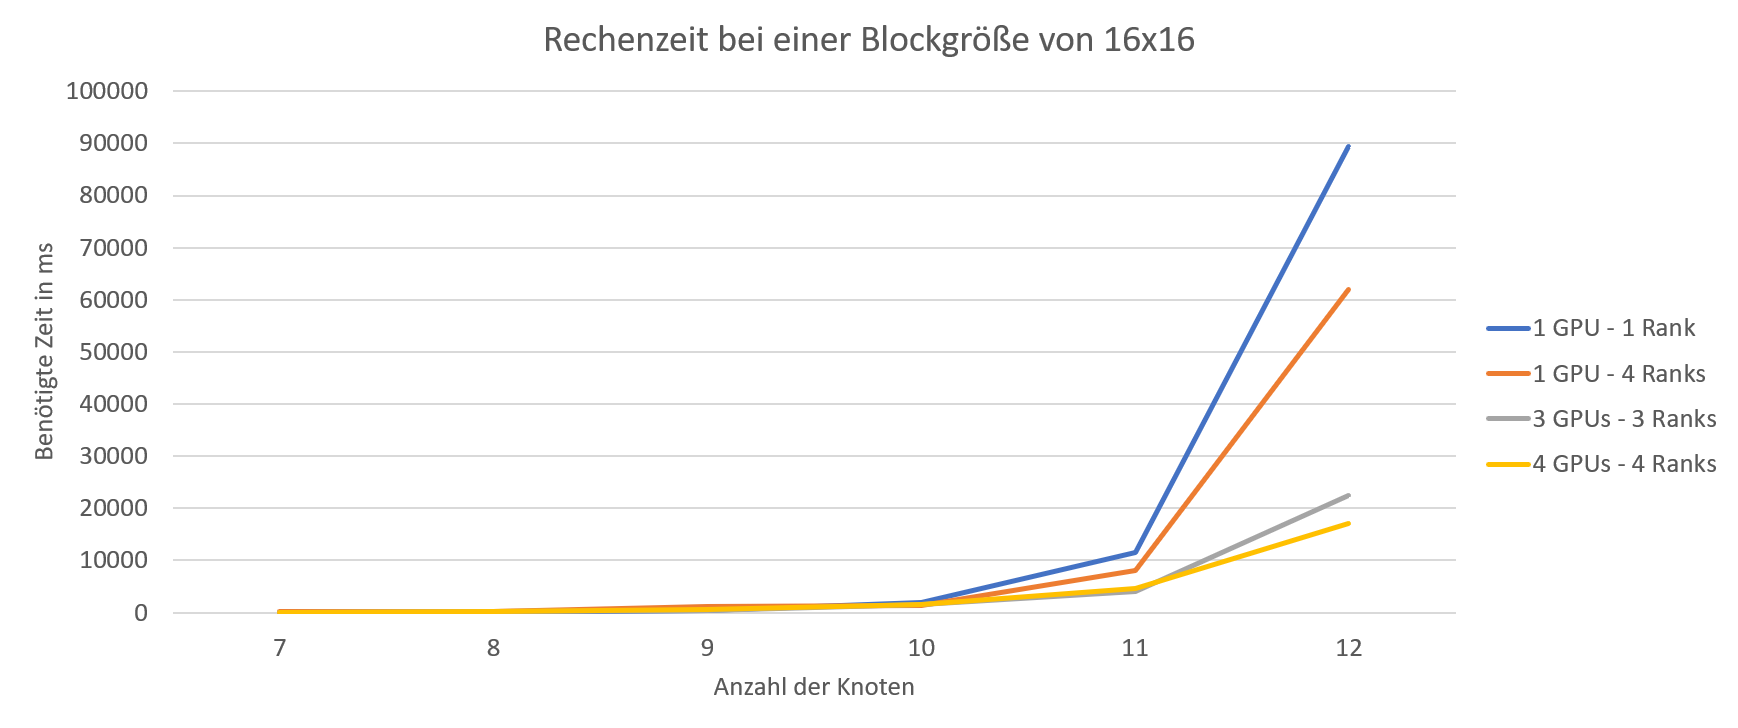
\includegraphics[width=1.0\textwidth]{images/Diagramm2.png}
	\caption{Grafische Darstellung der Rechenzeit der parallelen Implementierung des Floyd-Warshall-Algorithmus bei einer Blockgröße von 16x16}
	\label{img:dia1}
\end{figure}
\begin{figure}[H]
	\centering
	\captionsetup{justification=centering} 
	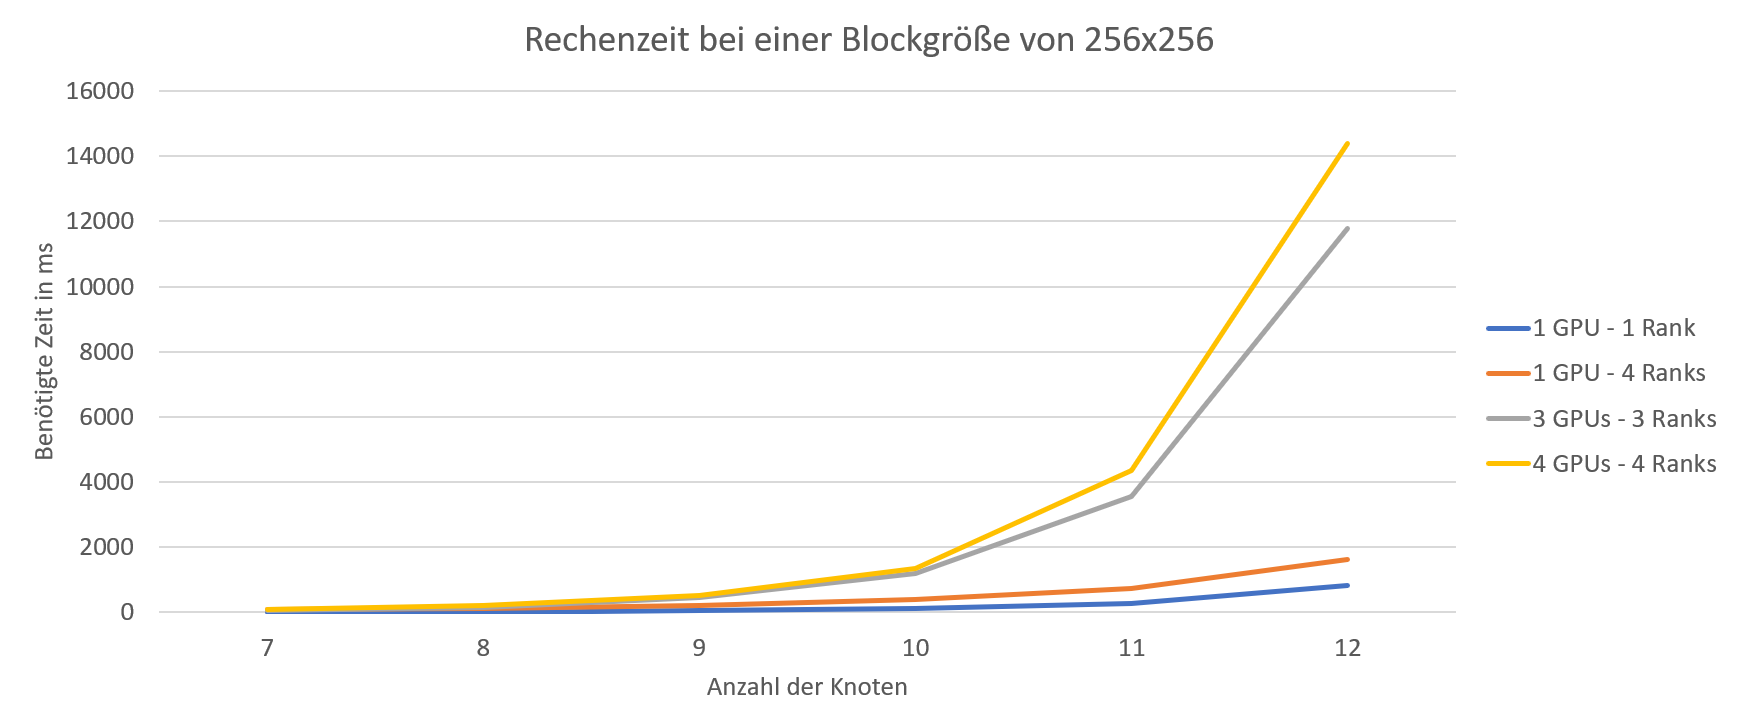
\includegraphics[width=1.0\textwidth]{images/Diagramm1.png}
	\caption{Grafische Darstellung der Rechenzeit der parallelen Implementierung des Floyd-Warshall-Algorithmus bei einer Blockgröße von 256x256}
	\label{img:dia2}
\end{figure}
\section{Zusammenfassung}
Wie die Ergebnisse des Benchmarks zeigen, ist je nach Größe und Art des Problems eine erhebliche Verringerung der benötigten Rechenzeit bei der Verwendung von mehreren Grafikchips zu erkennen. In Einzelfällen konnte die Rechenzeit dabei um ein Vielfaches reduziert werden. Nach wie vor ist es wichtig darauf hinzuweisen, dass die Verwendung von einem bzw. mehreren Grafikchips zur Berechnung eines Problems nicht immer von Vorteil ist. Dies ist grade im Hinblick auf die für die Kommunikation benötigte Zeit von Fall zu Fall abzuwägen. Die im Rahmen dieser Arbeit implementierten Algorithmen können auch von herkömmlichen Prozessoren schnell bearbeitet werden. Es ist anzunehmen, dass die Nutzung eines GPU-Clusters grade im Bereich des maschinellen Lernens erhebliche Vorteile bieten kann. 
\newpage
\addcontentsline{toc}{section}{\protect\numberline{}{Anhang}} 
\begin{appendix} 
\section{Aufbau des Clusters}
\begin{figure}
	\centering
	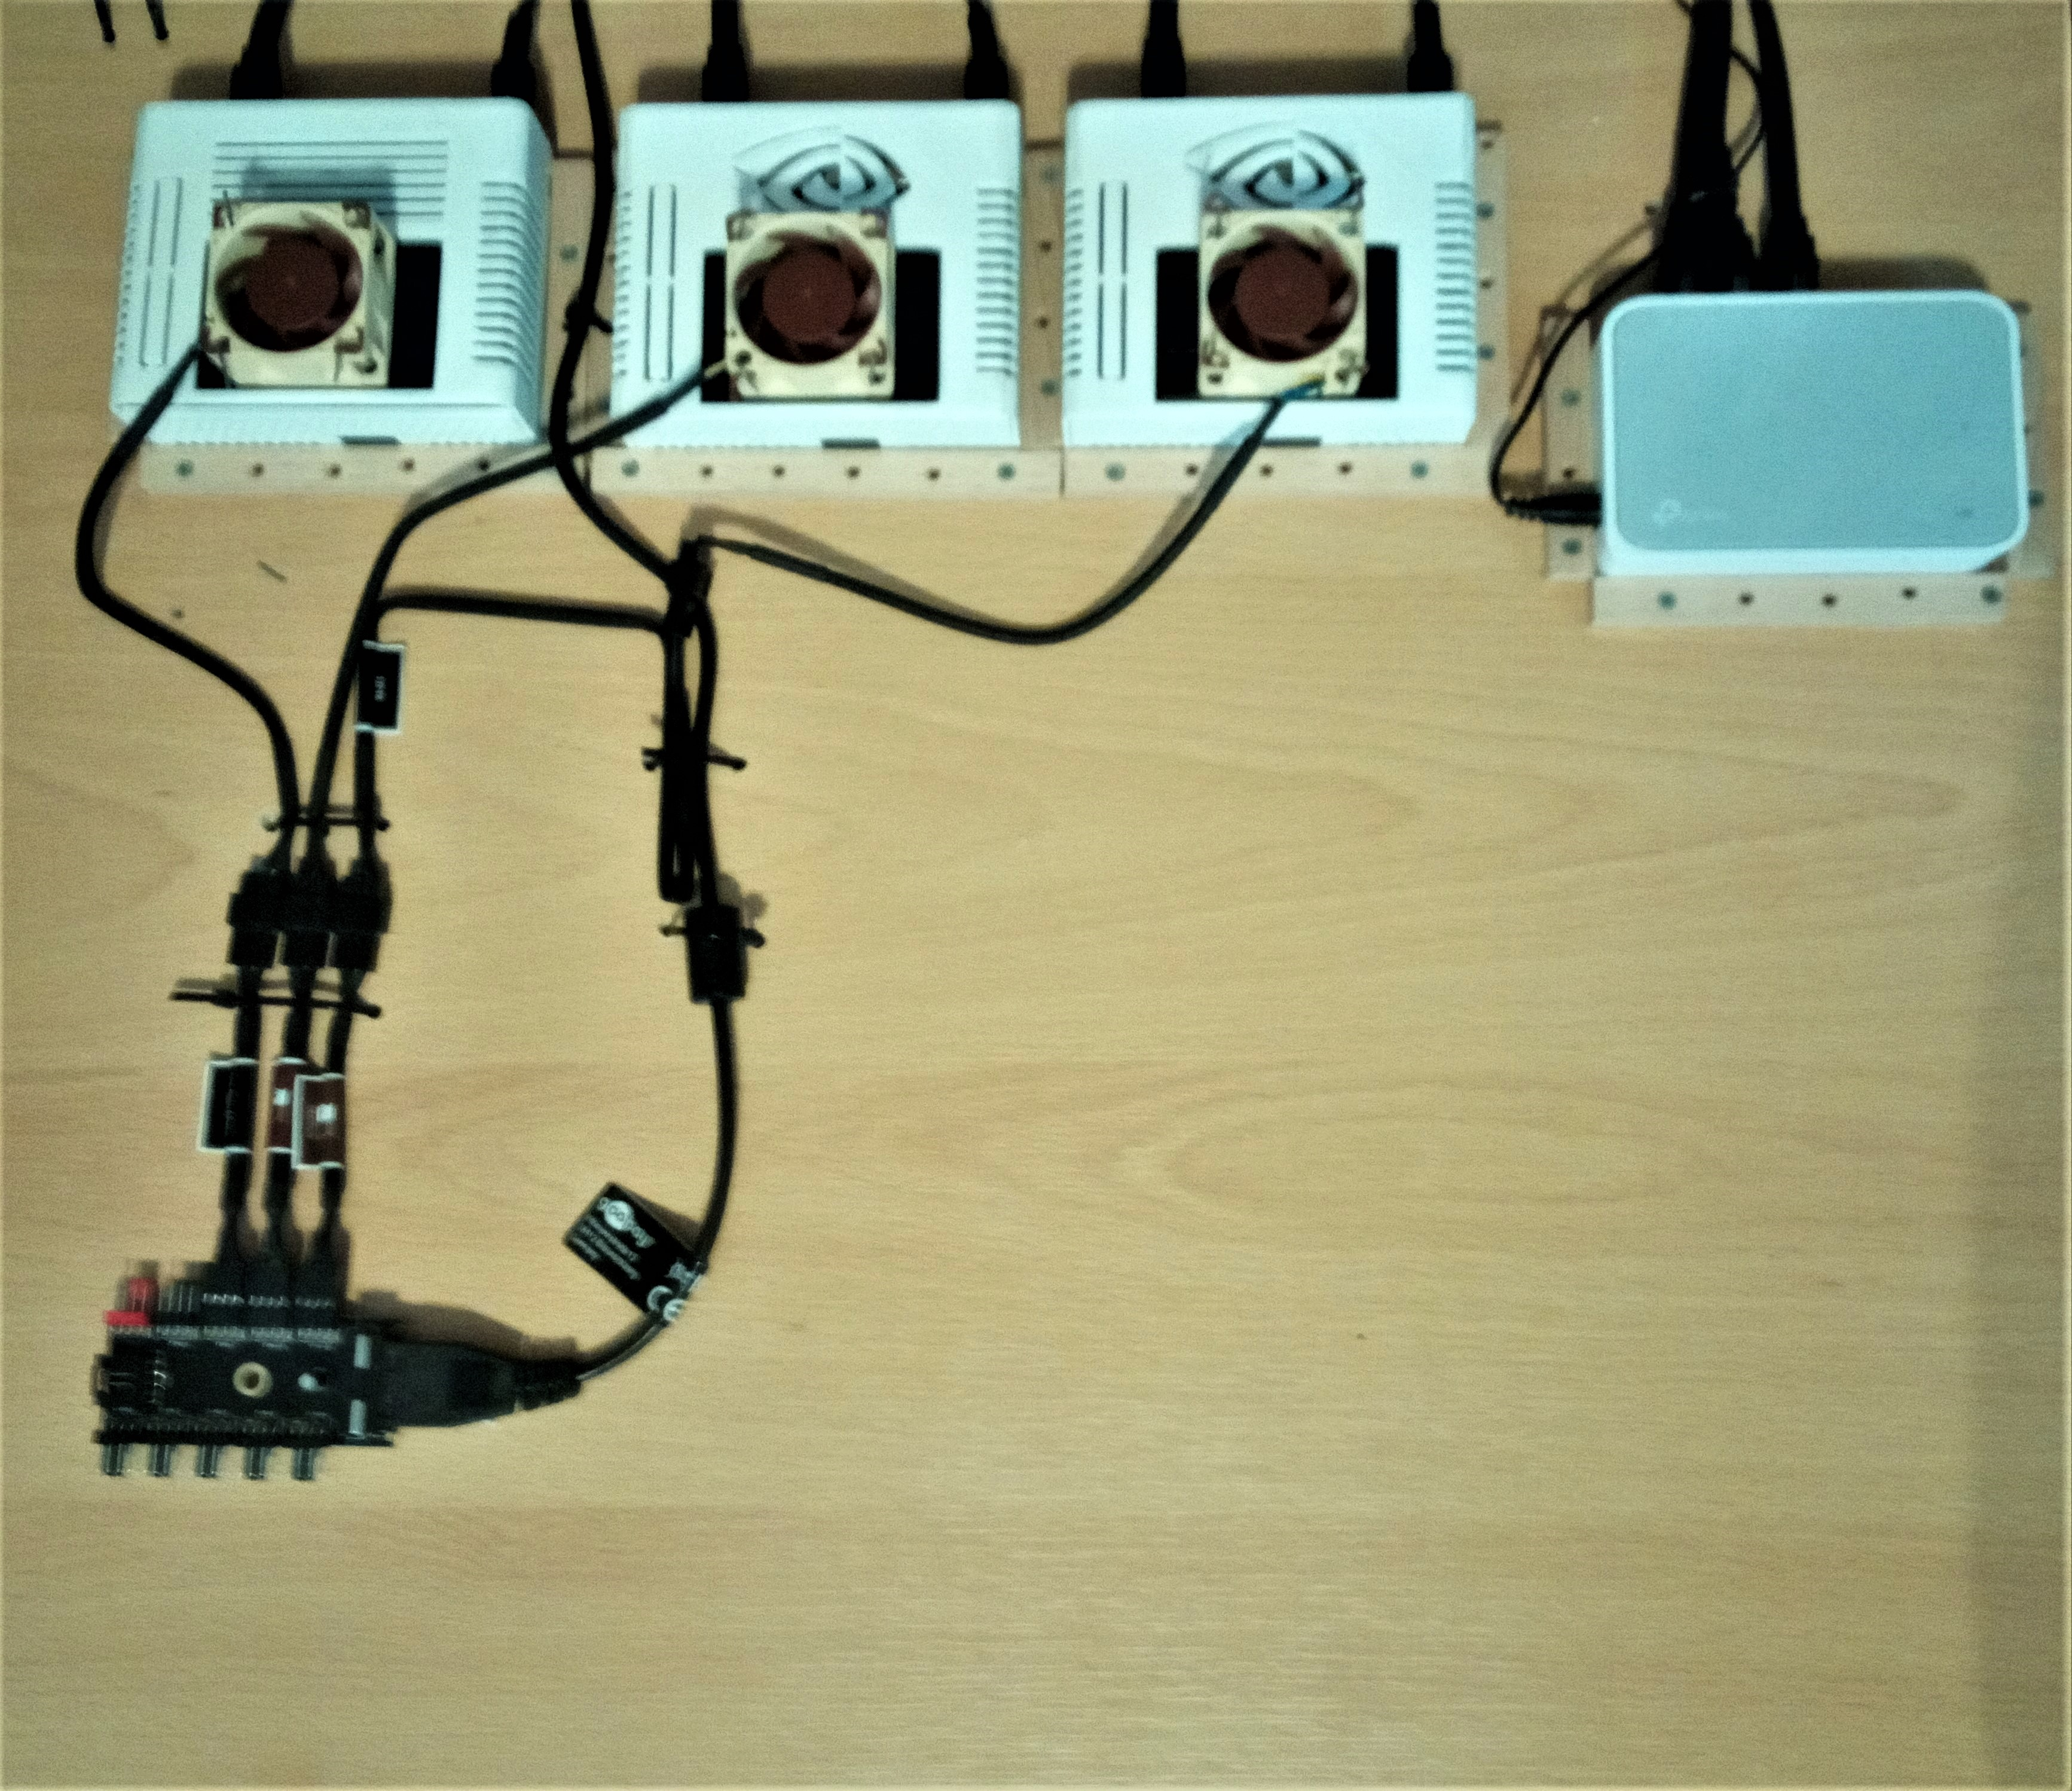
\includegraphics[width=1.0\textwidth]{images/Foto1.jpg}
	\caption{Der im Rahmen dieses Projektes erstellte Mini-Cluster. Zur besseren Nutzung wurden sowohl die Nvidia Jetson Nanos als auch der Switch durch seitliche Leisten auf einem Holzbrett fixiert. Um die vollständige Leistung durch die Nutzung des Powermodus zu erzielen, wurde desweiteren auf jedem Jetson Nano ein 40mm Lüfter installiert. Für die Steuerung dieser Lüfter wurde ein externer Lüfter-Controller genutzt, weil die Lüfter eine Betriebsspannung von 12V benötigen, der Jetson Nano jedoch nur Lüfter mit 5V Betriebsspannung unterstützt.}
	\label{img:foto1}
\end{figure}
\newpage
\section{Quellcode Vektoraddition}
\begin{CPP}
#include <cstdlib>
#include <algorithm>
#include <cmath>
#include <cstdio>
#include <string>

#include <mpi.h>
#include <unistd.h>

#define BLOCKSIZE 256

// Fehlerbehandlung

#define TRY(command) { cudaError_t cudaStatus = command; 
  if (cudaStatus != cudaSuccess) 
  {fprintf (stderr, "Error %d - %s\n", cudaStatus, 
  cudaGetErrorString(cudaStatus));
  goto Error; }}

// Berechnung der Summe zweier Vektoren

__global__ void sum(int n, float* x, float* y) {

	// Grid-Stride-Loop	

  	size_t const index = blockIdx.x * blockDim.x + threadIdx.x;
  	size_t const stride = blockDim.x * gridDim.x;
  	for (size_t i = index; i < n; i += stride) {

    		y[i] = x[i] + y[i];
  	}

	__syncthreads();
}


int main(int argc, char* argv[]) {
  	
	int N; // Groesse des Vektors

  	N = atoi(argv[1]); // Vektorgroesse aus Commandline-Paramter lesen

	// Check Input

	if (N <= 0) {

		printf("Die Vektorgroesse darf nicht Null oder negativ sein!");
		return EXIT_FAILURE;
	}

	
	
	// MPI-Init		

  	MPI_Init(&argc, &argv);

 	int MPIRank, MPISize;
  	MPI_Comm_rank(MPI_COMM_WORLD, &MPIRank);
  	MPI_Comm_size(MPI_COMM_WORLD, &MPISize);

	// Ueberpruefung, ob und wie viele cudafaehige Geraete vorhanden sind

  	int devicenumber;
  	cudaError cudaResult = cudaGetDeviceCount(&devicenumber);
  	if (cudaResult != cudaSuccess || devicenumber == 0) {

    		printf("Es wurden keine cudafaehigen Geraete gefunden!");
    		MPI_Finalize();
   		return EXIT_FAILURE;
  	}

	// Auslesen der Cuda-Device-Properties

  	for (int i = 0; i < devicenumber; ++i) {

    		cudaDeviceProp properties;
    		cudaGetDeviceProperties(&properties, i);
    		std::printf("Rank: %d CUDA device %d name: %s \n", MPIRank,
		   i, properties.name);
  	}

	// Definition der zwei Vektoren

  	float* x;
  	float* y;

	double MPIStart, MPIEnd, MPITimePassed;
	MPIStart = MPI_Wtime();

	// Initialisieren der Vektoren

  	if (MPIRank == 0) {

        	x = new float[N * MPISize];
      		y = new float[N * MPISize];
    
    		for (int i = 0; i < N * MPISize; ++i) x[i] = 1.f;
    		for (int i = 0; i < N * MPISize; ++i) y[i] = 2.f;
  	}	

  	int result;
	
	// Allokieren des Geraetespeichers; MPI-Scattering

  	float* d_x;
	float* d_y;

	// cudaMallocManaged fuer Unified Memory

  	cudaResult = cudaMallocManaged(&d_x, N * sizeof(float));
	cudaResult = cudaMallocManaged(&d_y, N * sizeof(float));	

  	if (cudaResult != cudaSuccess) {

    		printf("Fehler beim Allokieren von Cuda-Managed-Memory: 
^		  %s\n", cudaGetErrorString(cudaResult));
    		MPI_Finalize();
    		std::exit(EXIT_FAILURE);
  	}

  	result = MPI_Scatter(x,             // SendBuffer
                             N,             // SendCount
                             MPI_FLOAT,     // SendType
                             d_x,           // ReceiveBuffer
                             N,             // ReceiveCount
                             MPI_FLOAT,     // ReceiveType
                             0,             // Root
                             MPI_COMM_WORLD // Communicator
                            );


  	if (result != MPI_SUCCESS) {
    	
   		printf("Fehler beim MPI-Scattering");
    		MPI_Finalize();
    		std::exit(EXIT_FAILURE);
  	}


  	result = MPI_Scatter(y,             // SendBuffer
                             N,             // SendCount
                             MPI_FLOAT,     // SendType
                             d_y,           // ReceiveBuffer
                             N,             // ReceiveCount
                             MPI_FLOAT,     // ReceiveType
                             0,             // Root
                             MPI_COMM_WORLD // Communicator
                            );


  	if (result != MPI_SUCCESS) {
    	
   		printf("Fehler beim MPI-Scattering");
    		MPI_Finalize();
    		return EXIT_FAILURE;
  	}

	// Ermitteln der Blockanzahl	

  	int blocksize = BLOCKSIZE;
  	int blocknumber = (N + blocksize - 1) / blocksize;

	// Kernel

	float CUDATimePassed; // 
	cudaEvent_t CUDAStart, CUDAStop; // 
	
	TRY(cudaEventCreate(&CUDAStart));
	TRY(cudaEventCreate(&CUDAStop));
	TRY(cudaEventRecord(CUDAStart, 0));

	// Kernel

	sum<<<blocknumber, blocksize>>>(N, d_x, d_y);

  	cudaResult = cudaDeviceSynchronize();
  	if (cudaResult != cudaSuccess) {
	
        	printf("Fehler: Cuda asynchron: 
	  %s\n", cudaGetErrorString(cudaResult));
    		MPI_Finalize();
    		return EXIT_FAILURE;
  	}

	// Zeit-Benchmarking

	TRY(cudaEventRecord(CUDAStop, 0));
	TRY(cudaEventSynchronize(CUDAStop));
	TRY(cudaEventElapsedTime(&CUDATimePassed, CUDAStart, CUDAStop));

	MPI_Barrier(MPI_COMM_WORLD);
	MPIEnd = MPI_Wtime();
	MPITimePassed = MPIEnd - MPIStart;

	if (MPIRank == 0) {

		printf("\nBenoetigte Zeit Kernel: %3.1f ms \n", CUDATimePassed);
		printf("Gesamt benoetige Zeit: %f ms \n", MPITimePassed*1000);
	}

	

Error:

  	cudaFree(d_y);
  	cudaFree(d_x);

  	if (MPIRank == 0) {

    		delete[] y;
    		delete[] x;
  	}

  	MPI_Finalize();
  	return EXIT_SUCCESS;
}
\end{CPP}
\end{appendix}
\newpage
\bibliography{literatur}{}
\addcontentsline{toc}{section}{Literatur}  
\end{document}
